% Capitolo 2

\chapter{Reti federate eventualmente connesse}
\label{Capitolo2}
\lhead{Capitolo 2. \emph{Reti federate eventualmente connesse}}

Con rete federata si può intendere un universo molto ampio di
situazioni. In questo lavoro si considera sopratutto una rete federata
con le seguenti caratteristiche:

\begin{itemize}
  \item amministrazione decentrata 
  \item accesso alla gestione logica (e fisica) della rete
  \item conoscenze tecniche locali sulle tecnologie usate dalla rete
  \item servizi interni alla rete federata
  \item interazione tra reti locali intelligenti
\end{itemize} 

Una rete federata, quindi, intesa come un insieme di soluzioni
tecnicamente viabili ed adattabili ad usi, costumi e contesti
differenti, che permetta una gestione flessibile della rete, con
sotto-reti eterogenee, sfruttando diverse tecnologie, ad esempio P2P
ove necessario. Una rete federata si adatta particolarmente ad un
contesto dove esiste già una struttura organizzativa che si può
riflettere nella struttura di rete e che ne può accompagnare la
gestione.

\section{Reti federate eventualmente connesse}
L'introduzione sul contesto suggerisce l'ambito di ricerca ma
necessita una restrizione maggiore. Per ``rete federata eventualmente
connessa'', consideriamo, oltre alle premesse fatte, una rete federata
basata su connessioni non sempre disponibili, quali le connessioni
satellitari, con l'esigenza di mantenere i servizi federati attivi,
anche in assenza di comunicazione. I servizi federati sono inoltre
ottimizzati per la resilienza del sistema e la riduzione del traffico
di rete esterno, attraverso strategie di replicazione, sincronizzazione
e memorizzazione dei dati sull'infrastruttura logica/fisica locale.

\section{La Rete Mocambos}
\label{sec:ReteMocambos}

\begin{quote}
  ``\emph{É uma rede solidária de comunidades, no qual o objetivo
    principal é compartilhar idéias e oferecer apoio recíproco.}''
  \ldots ``\emph{A tecnologia é uma frente de trabalho da Rede
    Mocambos, sendo ao mesmo tempo idéia e meio para transferir
    idéias.}''\footnote{``è una rete solidale di comunità che ha come
    principale obbiettivo condividere idee e offrire appoggio
    reciproco'' \ldots ``La tecnologia è uno dei campi di attuazione
    della Rete Mocambos, essendo al tempo stesso idea e mezzo per
    trasferire idee.'', tradotto da
    \url{http://www.mocambos.net/sobre}.}, \citep{RMSobre}.
\end{quote}

La Rete Mocambos (RM), attualmente, coinvolge direttamente più di
duecento comunità quilombola, collettivi, comunità indigene e
\emph{terreiros}\footnote{Con il termine \emph{terreiros} vengono
  comunemente identificati i luoghi di culto delle religioni
  afro-brasiliane, quali Candomblé, Umbanda, Xamba etc.} (vedi figura
\ref{fig:MappaRedeMocambos}). Esistono due accordi\footnote{Gli
  accordi sono stati firmati, a nome della Rete Mocambos, dalla
  \emph{Casa de Cultura Tainã}.} tra la Rete Mocambos e il Ministero
delle Comunicazioni, all'interno del programma GESAC e del programma
Telecentros.BR.

\begin{figure}[htbp]
  \centering
  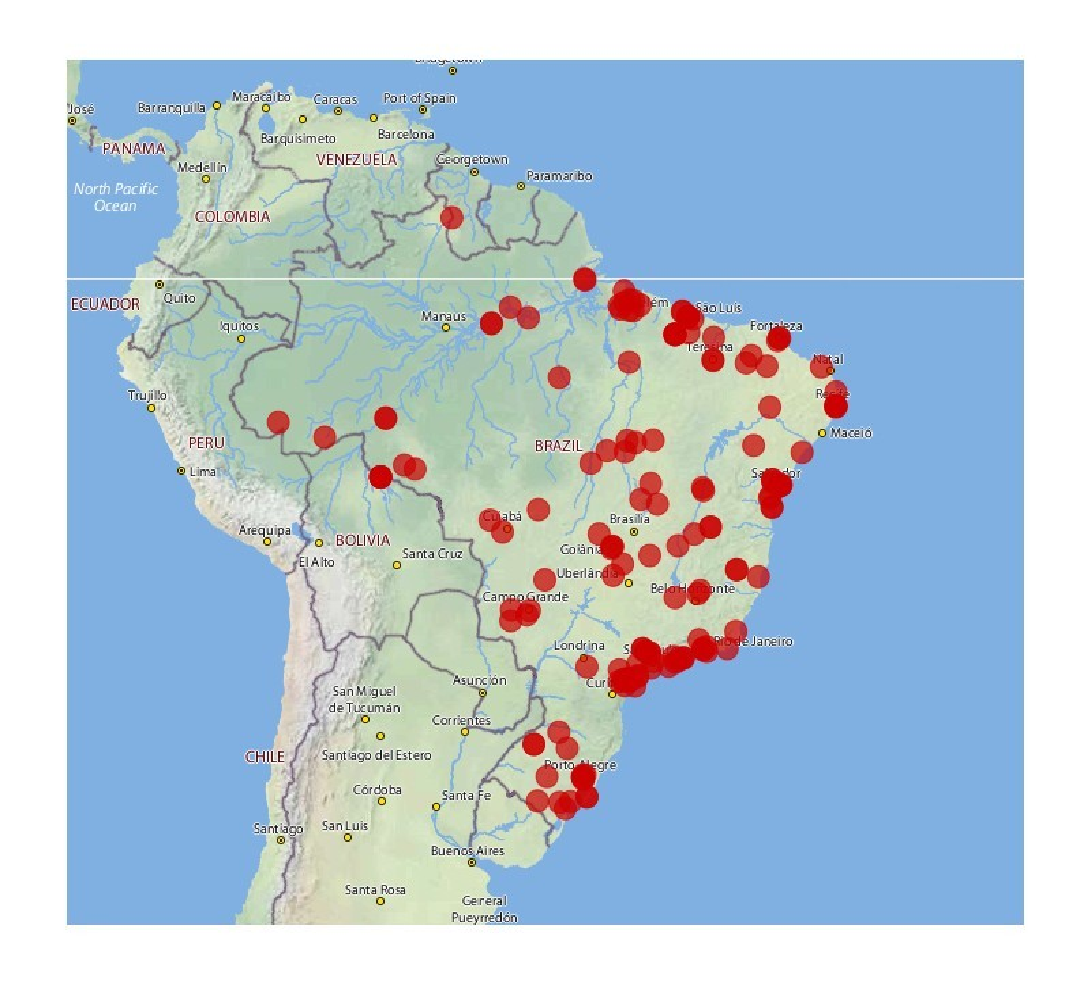
\includegraphics[width=\textwidth]{./Figure/MappaRedeMocambos.pdf}
  \rule{35em}{0.5pt}
  \caption[Mappa delle comunità della Rete Mocambos, tratto da
  \url{http://mapa.mocambos.net}]{Mappa delle comunità della Rete
    Mocambos, tratto da \url{http://mapa.mocambos.net}}
  \label{fig:MappaRedeMocambos}
\end{figure}

Il GESAC garantisce connettività satellitare a tutte le comunità, con
una banda limitata dovuta al tipo di tecnologia, non facilmente
sostituibile nel breve e medio termine. Tramite il programma
Telecentros.BR sono in corso di installazione dei \emph{telecentros},
sale attrezzate con computer ad accesso pubblico, e saranno erogate
borse per tutor locali, per la gestione degli spazi. Proprio in un
contesto così specifico nasce la necessità di adattare la tecnologia
alle esigenze locali, anche per le limitazioni tecniche imposte. La
scarsità di banda spinge a riconsiderare la rete non solo come il
mezzo di connessione verso i grandi \emph{data center}. La rete può, e
in questo caso deve, essere strutturata nel territorio con logiche di
sviluppo e gestione localmente determinate dalla comunità. In questo
senso è indispensabile la formazione e l'accesso alle tecnologie. La
\emph{Casa de Cultura Tainã}, nucleo fondatore della RM, è tra le
prime realtà popolari che hanno percepito la necessità del Software
Libero, come espressione della libertà di poter creare i propri
strumenti tecnologici digitali. L'esclusione digitale non riguarda
solo l'accesso al mondo digitale ma l'impossibilità di contribuire
alla sua creazione e crescita.

\begin{figure}[htbp]
  \centering
  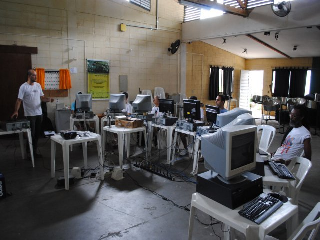
\includegraphics[width=\textwidth]{./Figure/taina_oficina.pdf}
  \rule{35em}{0.5pt}
  \caption[Laboratorio di grafica 3D con Blender alla \emph{Casa de
    Cultura Tainã}]{Laboratorio di grafica 3D con Blender alla
    \emph{Casa de Cultura Tainã}}
  \label{fig:oficinaBlender}
\end{figure}

Per la RM è importante, sotto molti aspetti, poter costruire e gestire
i mezzi di comunicazione e adattarli al loro contesto. In Brasile,
sono molte le comunità indigene, quilombola e
``tradizionali''\footnote{Per comunità tradizionali si intende
  comunità con culture e società proprie, per lo più di origine
  afro-indigena, situate spesso in ambito rurale e fortemente legate
  alla natura. La costituzione brasiliana sancisce il diritto alla
  terra per le comunità indigene e quilombola, e lo stato deve
  tutelare e garantire la diversità culturale.} che conoscono bene le
potenzialità delle tecnologie digitali e stanno, via via, cominciando
a dominarle. Ciò non sarebbe stato possibile senza l'esistenza e
l'ampia disponibilità di Software Libero. Tecnologie digitali sotto
forma di prodotti commerciali sarebbero un ennesimo passo verso la
dipendenza economica e culturale. Questa consapevolezza è alla base di
scelte ben ponderate. Ricordo che, qualche anno fa, a Brasilia,
durante una riunione del programma del governo federale \emph{Luz para
  Todos}, programma per fornire elettricità anche alla popolazione in
zone rurali e amene, un \emph{cacique}\footnote{ \emph{Cacique} è un
  termine con cui si definiscono i capi di alcune comunità indigene in
  America latina. } fece presente, che pur volendo l'energia
elettrica, questa dovesse essere limitata solo agli spazi comunitari e
non alle case. Non è difficile intuire il perché di tale
condizione. Oltre agli aspetti culturali, avere un contatore e una
bolletta per ogni casa significherebbe introdurre costi in denaro, che
non sono compatibili con la loro economia.

% \section{DA RIVEDERE}
% Una rete federata deve essere gestita. Servono risorse e conoscenze
% locali. Questo comporta un investimento strategico che riguarda
% aspetti ecomomici, ma sopratutto umani. E' necessaria una formazione
% continua e personale preparato per la gestione. Il mercato ha escluso
% questo modello anche per i suoi costi. Gli attori principali della
% new-economy globale sono riusciti a rendere questo passaggio quasi
% naturale, offrendo sistemi altamente funzionali e a condizioni
% particolarmente appetibili. Inanzitutto i servizi sono gratuiti e
% questo è la base per renderne l'uso in massa possibile. Da un punto di
% vista tecnico-informatico, la diffusione di servizi internet modello
% ToS vincenti, ha provocato una migrazione in massa delle maestrie del
% settore, sopratutto le nuove generazioni, verso lo sviluppo basato su
% API et similia.

% Passando dai protocolli di comunicazione standard alle API/ToS, dalla
% gestione della rete all'accesso al cloud, si p le conoscenze e
% sopratutto la ricerca

% (RITORNARE A DIRE PERCHE LE RETI FEDERATE SONO INTERESSANTI. SERVE UNA
% SCELTA POLITICA PER RIPRENDERE IL POSSESSO DELLA RETE COME SPAZIO
% TECNOLOGICO NON SOLO COME CONNESSIONE A POCHI CLOUD E DATACENTER)
% . Inoltre la programmazione di rete via API ha reso gli orizzonti in
% buona parte predeterminati dalle imprese madri del servizio.

% I nuovi mezzi di comunicazione offrono evidenti vantaggi, a cui non
% possiamo più rinunciare, tanto da spingere le Nazioni Unite a
% riconoscere l'accesso a internet come un diritto fondamentale \ref{}.

% Consideriamo in particolare una rete di servizi federati tra molte
% reti locali (attualmente circa 200 per la Rede Mocambos). La
% restrizione, oltre a essere dettata da un vincolo reale (la Rede
% Mocambos è basata su connessioni satellitari), può rappresentare un
% punto di partenza per ampliare la ricerca verso reti locali
% intelligenti e più sostenibili. Anche la diffusione di reti mesh ha
% risvegliato l'interesse per le reti di servizi federati su risorse
% decentralizzate e gestite localmente.


\section{Tecnologie}
Prima di addentrarci nei requisiti specifici, e nelle scelte adottate,
può essere utile una breve rassegna degli strumenti tecnologici presi
in considerazione per strutturare il prototipo per la Rete Mocambos di
rete federata eventualmente connessa, in particolare per i suoi
servizi di base, quali identificazione, autenticazione e
messaggistica.

\subsection{LDAP}
Lightweight Directory Access Protocol (LDAP) è un insieme di
protocolli aperti per accedere a informazioni conservate centralmente
attraverso una rete. LDAP organizza le informazioni attraverso una
gerarchia ad albero chiamata Directory Information Tree (DIT). LDAP è
un sistema client/server. Il server può usare una varietà di database
per conservare un DIT, normalmente ottimizzati per le operazioni di
lettura. Quando un'applicazione client si collega ad un server LDAP,
può sia interrogare la directory che cercare di modificarla. Nel caso
in cui si verifica una interrogazione, il server può rispondere in
modo locale, oppure può inoltrare la richiesta ad un server LDAP che
sia in possesso di una risposta. Se l'applicazione di un client stà
cercando di modificare le informazioni all'interno di una directory
LDAP, il server verifica se l'utente possiede il permesso di
effettuare il cambiamento, e successivamente aggiunge o aggiorna le
informazioni. LDAP supporta la delega di parte del DIT a server
specifici, la replica in sola lettura e la replica in
lettura/scrittura (multi-master).  LDAP è un protocollo solido, molto
diffuso e supportato, e da tempo è lo standard de facto per gestire
basi di dati di utenti. OpenLDAP è una implementazione aperta e libera
del protocollo LDAP, che include client, server e una serie di
strumenti per facilitarne l'amministrazione.

\subsection{XMPP}
Extensible Messaging and Presence Protocol (XMPP) è un insieme di
protocolli aperti per la messaggistica e la presenza in rete basato su
XML. XMPP è un sistema client/server. Le specifiche per la
comunicazione tra server fanno si che gli utenti di un server possono
interagire in modo trasparente con gli utenti di altri server
federati. La XMPP Standards Foundation (XSF), coordina lo sviluppo
delle estensioni dello standard tramite le XMPP Extension Protocols
(XEPs), che ad oggi sono ben 311. XMPP e le XEPs costituiscono una
ambiente flessibile e completo per lo sviluppo di servizi
federati. Questi protocolli sono gia utilizzabili grazie a moltissime
implementazioni di server, client e librerie libere. Anche la storia
di XMPP, un tempo noto come Jabber, è interessante. Jabber venne
infatti inizialmente sviluppato da Jeremie Miller nella sua fattoria
nell'Iowa. E' un esempio concreto di come la ricerca e lo sviluppo di
tecnologie della comunicazione, fuori da ambiti accademici e
imprenditoriali, oltre che possibile può essere rivoluzionaria. Oggi
infatti XMPP è la tecnologia più usata per la messaggistica anche dai
grandi attori della new economy.

Per le necessità specifiche di una rete è possibile quindi estendere e
personalizzare le funzionalità del proprio server XMPP e al tempo
stesso usufruire dei servizi base, messaggistica e presenza,
implementanti dai server già esistenti in rete.

\subsection{OpenID}
OpenID è un sistema di identificazione decentralizzato nel quale la
propria identità è un URL che può essere verificata da qualunque
server supporti il protocollo. E' un protocollo aperto e sono
disponibili varie implementazioni libere. Inoltre il protocollo è
stato adottato dai principali fornitori di servizi web. Con OpenID è
possibile usare la stessa identità su piu servizi ed è un ottima base
per un sistema Single Sign On (SSO). Il protocollo sfrutta HTTP e e
Cookies per mantenere una sessione attiva. Al primo tentantivo di
autenticazione presso un servizio compatibile con OpenID, si viene
reindirizzati verso il proprio provider OpenID per effetturare
l'accesso e confermare l'autorizzazione a procedere al servizio
iniziale. Per tutta la durata della sessione, è possibile accedere ai
servizi OpenID senza reinserire le credenziali.

\begin{figure}[htbp]
  \centering
  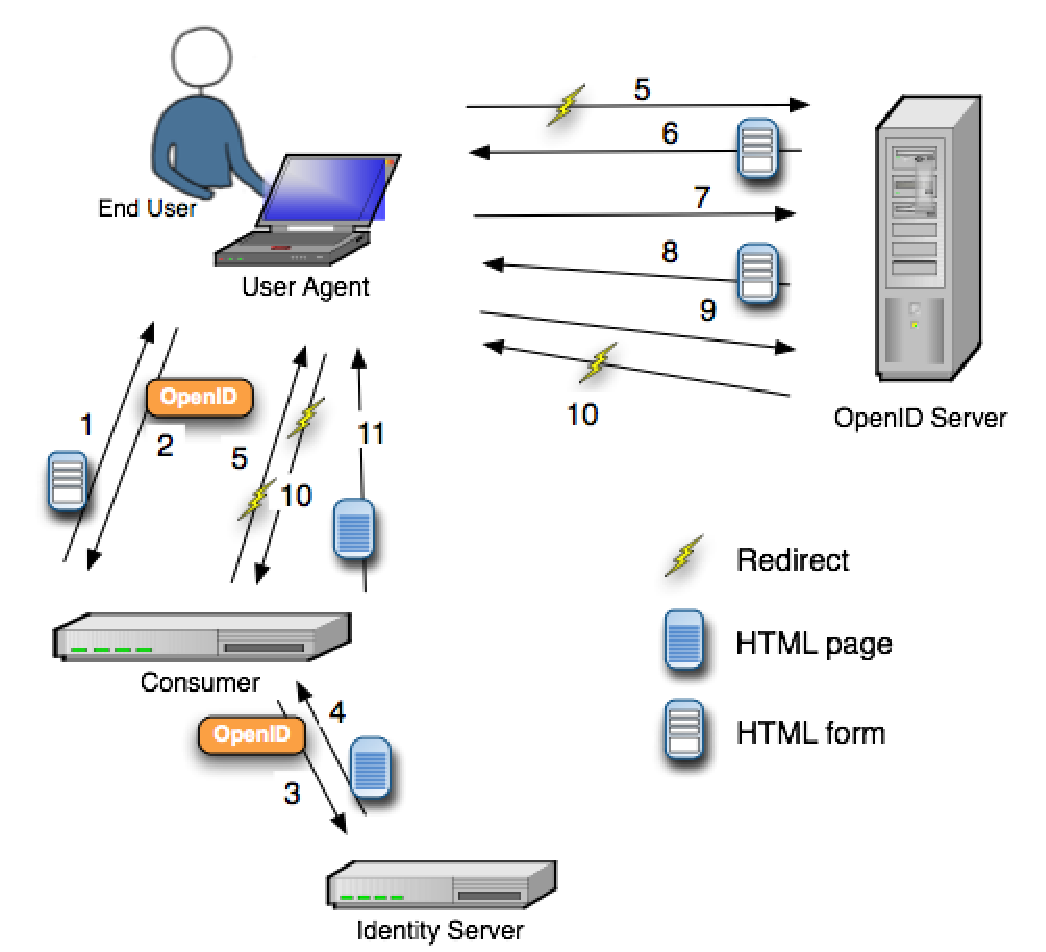
\includegraphics[width=0.6\textwidth]{./Figure/OpenID_Scenario.pdf}
  \rule{35em}{0.5pt}
  \caption[Diagramma di autenticazione di OpenID]{Diagramma di autenticazione di OpenID}
  \label{fig:OpenID}
\end{figure}



\subsection{OAuth}
OAuth è un protocollo aperto per l'autorizzazione di servizi tramite
API. Ad esempio, permette ad un utente di dare l'accesso alle sue
informazioni presenti su un sito detto service provider, ad un altro
sito, chiamato consumer, senza però condividere la sua identità. E' un
metodo per pubblicare e interagire con dati protetti. Esistono molti
altri protocolli e API simili come Google AuthSub, AOL OpenAuth, Yahoo
BBAuth, Upcoming API, Flickr API, Amazon Web Services e ognuno
fornisce dei metodi proprietari per lo scambio di credenziali e per
l'accesso tramite token. OAuth è una standardizzazione aperta delle
pratiche piu diffuse. Inoltre è stato pensato per il supporto a vari
tipi di applicazioni, non soltanto per i servizi web.


\subsection{Shibboleth}
Shibboleth è un architettura e un implementazione aperta per
l'autenticazione e autorizzazione di identità federate basata su
Security Assertion Markup Language (SAML). Le identità federate
permettono che le informazioni di un utente sotto un certo dominio
possano essere condividise con un altro dominio federato. Questo
permette il SSO attraverso piu domini senza lo scambio di nomi utente
e password. Gli IdP mantengono le informazioni sull'utente mentre i SP
fanno uso di queste informazioni per l'accesso sicuro ai contenuti.

\subsection{Kerberos}
Kerberos è un protocollo aperto per l'autenticazione forte in reti di
computer. E' un protocollo client/server e consente l'autenticazione
reciproca, ossia entrambi verificano le loro identità. Kerberos è
basato sul protocollo di Needham-Schroeder a chiavi simmetriche e
prevede un entità terza di fiducia chiamata Key Distribution Center
(KDC).

\subsection{Django}\label{Django}
Django è un framework, scritto in Python, per lo sviluppo rapido di
applicazioni web, anche conosciuto come ``\emph{The web framework for
  perfectionists with deadlines}''\footnote{``Il framework web per i
  perfezionisti con scadenze''.}, poichè è stato creato con l'obiettivo
di aderire il più possibile al principio DRY\footnote{``Don't Repeat
  Yourself (DRY, anche conosciuto come ``Single Point of Truth'') è un
  principio secondo il quale l'informazione non debba essere ripetuta
  e ridondante e non si debba esprimere lo stesso concetto più di una
  volta, specie se in forma diversa'', tratto da Wikipedia:
  \url{http://it.wikipedia.org/wiki/Don\%27t_Repeat_Yourself}.}, e
quindi fornisce tutti gli strumenti per scrivere codice pulito in modo
pragmatico ed efficace.

Le caratteristiche di Django sono le seguenti:
\begin{itemize}
\item Django è un framework \emph{Model, View, Template}, (MVT),
  corrispondente al diffuso pattern \emph{Model, View, Controller},
  (MVC). Il \emph{Template} di Django corrisponde alla \emph{view} in
  un qualunque framework MVC, mentre la \emph{View} corrisponde al
  \emph{controller} (anche se le funzionalità del \emph{controller},
  nel caso di Django, non sono limitate alla componente \emph{View}).
\item Django consente di modellare i dati direttamente in python e l'
  \emph{Object Relational Mapper}, (ORM), si occupa di trasformarli in
  codice SQL. Allo stesso modo non serve scrivere query direttamente
  in SQL; basta usare l'ORM per avere i risultati direttamente
  restituiti come oggetti python. L'ORM di Django supporta PostgreSQL,
  MySQL, sqlite, Microsoft SQL Server ed Oracle.
\item Django possiede una libreria per i \emph{forms} davvero potente ed
  espressiva, che consente di realizzare logiche complesse in poche
  righe di codice, lasciando il massimo controllo allo sviluppatore su
  ogni aspetto.
\item Django è un framework ``\emph{batteries included}'', ovvero
  contiene al suo interno alcune applicazioni, dette \emph{apps}, per
  le funzionalità più comuni che dimezzano il tempo di sviluppo, ad
  esempio un sistema di autenticazione, una interfaccia
  amministrativa, un framework per generare le \emph{sitemaps XML} e
  molto altro. Inoltre la \emph{community} è piuttosto attiva ed
  esistono molte \emph{apps} da adattare e riutilizzare.
\item Django è tra i migliori framework per quanto riguarda la
  documentazione ufficiale. Oltre ad alcuni tutorial, utili per
  impararne le basi, quasi ogni aspetto del framework è documentato in
  modo eccellente.
\end{itemize}

\subsection{Git}\label{sec:GIT}
Git è un sistema multi-piattaforma per il controllo delle versioni
distribuito, progettato per essere rapido e usabile anche in grandi
progetti.

Le caratteristiche principali includono:
\begin{itemize}
\item è totalmente distribuito e ogni clone di un
  \emph{repository} contiene l'intero storico delle versioni su cui
  possono essere effettuate operazioni indipendentemente da
  connessioni di rete o da server centrali. Le modifiche possono
  essere copiate da una clone all'altro e vengono mantenute su
  \emph{branch} diversi, facilitando le operazioni di \emph{merge}. I
  \emph{repository} sono facilmente accessibili tramite l'efficiente
  protocollo di Git che, oltre a supportare l'HTTP, può funzionare in
  combinazione con SSH, per avere connessioni sicure e un sistema di
  autenticazione solido e diffuso.
\item supporta il \emph{branching}, ramificazione, e il
  \emph{merging}, fusione, in modo rapido e conveniente, includendo
  una serie di strumenti per visualizzare e navigare lo storico non
  lineare delle versioni.
\item è molto veloce e scala bene quando si lavora con progetti
  molto grandi e con molte modifiche, grazie ad un efficiente sistema
  di pacchettizzazione e memorizzazione dello storico (è considerato
  il più efficiente tra i sistemi attualmente disponibili).
\item assegna un nome di versione, per ogni \emph{commit},
  che è funzione dell'intero storico, per cui una volta pubblicata una
  versione, non è possibile alterare le vecchie senza essere
  notati. Inoltre le versioni possono essere etichettate e firmate
  digitalmente tramite GPG.
\end{itemize}

Git è un sistema completo che, in buon stile Unix, è organizzato in
programmi e comandi indipendenti, pensati per essere facilmente
usabili, sia automaticamente tramite \emph{scripting} sia in modo
interattivo dall'utente finale. Git è, quindi, una base solida per lo
sviluppo di applicazioni orientate alla sincronizzazione, alla
portabilità, e alla gestione autonoma e decentrata.

